%%%%%%%%%%%%%%%%%%%%%%%%%%%%%%%%%%%%%%%%%
% Frequently Asked Questions
% LaTeX Template
% Version 1.0 (22/7/13)
%
% This template has been downloaded from:
% http://www.LaTeXTemplates.com
%
% Original author:
% Adam Glesser (adamglesser@gmail.com)
%
% License:
% CC BY-NC-SA 3.0 (http://creativecommons.org/licenses/by-nc-sa/3.0/)
%
%%%%%%%%%%%%%%%%%%%%%%%%%%%%%%%%%%%%%%%%%

\documentclass[11pt]{article}

\usepackage[margin=1in]{geometry} % Required to make the margins smaller to fit more content on each page
\usepackage[linkcolor=blue]{hyperref} % Required to create hyperlinks to questions from elsewhere in the document
\hypersetup{pdfborder={0 0 0}, colorlinks=true, urlcolor=blue} % Specify a color for hyperlinks
\usepackage{todonotes} % Required for the boxes that questions appear in
\usepackage{tocloft} % Required to give customize the table of contents to display questions
\usepackage{microtype} % Slightly tweak font spacing for aesthetics
\usepackage{palatino} % Use the Palatino font
\def\ave#1{\left\langle#1\right\rangle}
\usepackage{amsmath}

\graphicspath{ {Figures/} }

\newcommand\textbox[1]{%
  \parbox{.6\textwidth}{#1}%
}

\setlength\parindent{0pt} % Removes all indentation from paragraphs

% Create and define the list of questions
\newlistof{questions}{faq}{\large Table of contents} % This creates a new table of contents-like environment that will output a file with extension .faq
\setlength\cftbeforefaqtitleskip{4em} % Adjusts the vertical space between the title and subtitle
\setlength\cftafterfaqtitleskip{1em} % Adjusts the vertical space between the subtitle and the first question
\setlength\cftparskip{.3em} % Adjusts the vertical space between questions in the list of questions

% Create the command used for questions
\newcommand{\class}[1] % This is what you will use to create a new question
{
\refstepcounter{questions} % Increases the questions counter, this can be referenced anywhere with \thequestions
\par\noindent % Creates a new unindented paragraph
\phantomsection % Needed for hyperref compatibility with the \addcontensline command
\addcontentsline{faq}{questions}{#1} % Adds the question to the list of questions
\todo[inline, color=green!40]{\textbf{#1}} % Uses the todonotes package to create a fancy box to put the question
\vspace{1em} % White space after the question before the start of the answer
}

% Uncomment the line below to get rid of the trailing dots in the table of contents
%\renewcommand{\cftdot}{}

% Uncomment the two lines below to get rid of the numbers in the table of contents
%\let\Contentsline\contentsline
%\renewcommand\contentsline[3]{\Contentsline{#1}{#2}{}}

\begin{document}

%----------------------------------------------------------------------------------------
%	TITLE AND LIST OF QUESTIONS
%----------------------------------------------------------------------------------------

\begin{center}
\Large{\bf Documentation for minimum Hubble variance program} % Main title
\end{center}

\listofquestions % This prints the subtitle and a list of all of your questions

\newpage % Comment this if you would like your questions and answers to start immediately after table of questions

%----------------------------------------------------------------------------------------
%	QUESTIONS AND ANSWERS
%----------------------------------------------------------------------------------------

\class{Getting started}\label{getting_started}

The program is structured into folders for 
\begin{itemize}
\item {\bf src} source (.cpp files)
\item {\bf include} header (.hpp) files
\item {\bf Figures} python plotting routines and generated figures
\item {\bf build} folder to store compiled code and executables
\item {\bf Documentation} the folder where this file is
\end{itemize}

To begin with navigate into the build folder and type:\\
\begin{verbatim}
cmake ..
make
\end{verbatim}

this will compile the code.  On OSX type equivalently:
\begin{verbatim}
cmake -DCMAKE_CXX_COMPILER=/usr/local/bin/g++ 
-DCMAKE_C_COMPILER=/usr/local/bin/gcc ..
\end{verbatim}

The executables which are compiled can be controlled in the CMakeLists.txt files, by commenting out (\#) the ``add executable" line for the corresponding source files.


%------------------------------------------------

\class{Classes}\label{classes}

The program is separated into the following classes

\begin{itemize}
\item \hyperref[get_data]{{\bf Get data} } loads in the relevant galaxy data
\item \hyperref[hvar]{\bf Hvar} calculates the Hubble flow and all associated parameters
\item \hyperref[boost_offset]{\bf Boost offset} compares two Hvar objects and determines the systematic boost offset
\item \hyperref[scanner]{\bf Scanner} contains the scanning routines
\item \hyperref[figures]{\bf Figures} contains all the functions for generating figures
\end{itemize}

\class{Get data}\label{get_data}

The get data class is used to load in the CF2 or COMPOSITE data sets.  Once initiated this object can be passed to any other calculations within the minvar program.  So far we have the capability to load in only these two samples, and if a new sample is added one must edit the corresponding source and header files depending on the structure of the new data file, although this should be trivial to copy the existing structure of the code.\\

An instance of the data object, in this case with the local name ``data" is initiated using the command
\begin{verbatim}
Get_data data
\end{verbatim}
followed by either
\begin{verbatim}
get_COMPOSITE();
\end{verbatim}
for the COMPOSITE sample or
\begin{verbatim}
get_CF2();
\end{verbatim}
for the CF2 sample.


\class{Hvar}\label{hvar}

This object contains the calculation of the Hubble constant in spherical shells along with all related quantities.  A general hvar object has the following quantities available for each shell
\begin{align*}
H_s, \ \ \ \sigma_{H,s}, \ \ \  \ave{r}_s, \ \ \ \ave{r^2}_s, \ \ \ \sigma_{\ave{r^2},s}, \ \ \ \Delta H_s,\ \ \  \sigma_{\Delta H,s}
\end{align*}
along with other parameters related to the number of shells and inner cutoff.\\

\textbf{Object initiation}

An instance of an hvar object, called ``hvar" here, is initiated with the code
\begin{verbatim}
Hvar hvar(data)
\end{verbatim}
with the data object defined above.\\

We are interested in calculating the hvar object in a frame of reference boosted with respect to the CMB.  There are two ways we can define the direction of the boost.  We can define the boost at the time of initiation of the Hvar object, using 
\begin{verbatim}
Hvar hvar(data, v_ref , l_ref , b_ref )
\end{verbatim}
where $(v_{ref},l_{ref},b_{ref})$ is the direction and magnitude of the boost with respect to the sun.  If this option is not used (and the plain constructor above is used instead), the frame is defined to the LG frame by default.\\

Alternatively we can use the command
\begin{verbatim}
hvar.set_direction(v, l, b)
\end{verbatim}
where hvar is the local name of the Hvar object and $(v,l,b)$ is the boost with respect to the reference boost $(v_{ref},l_{ref},b_{ref})$, or simply the LG if no reference boost was defined.\\

These two ways of defining the boost direction and magnitude are useful for different purposes.  We may wish to make many boosts with respect to ``some frame", so it is simple to define this ``some frame" once at the beginning and then make boosts with respect to this using the set direction command.  However, if simply comparing two frames there is degeneracy in how this is done.  It may also be convenient to have the choice of either boosting with respect to the LG (by using the set direction) or with respect to the sun (by setting the boost at the point of initiation).\\

\textbf{Choice of frame configuration}

We are free to choose the inner cutoff and the number of shells.  Extensive testing has only been done so far using 11 shells, and an inner cutoff of either 0 Mpc/$h$ (since we assume that all data below 2 Mpc/$h$ has been removed from the data file in the fist place) or 6.25 Mpc/$h$.  The specification of these choices takes place when we actually fill the Hvar object, using the command

\begin{verbatim}
calc_hvar(minr, nb)
\end{verbatim}

where minr and nb are the inner cutoff and number of shells respectively.  We can add more shells, if we want a final Hvar object that consists of both unprimed and primed shells, for example.  This can be done by using the command
\begin{verbatim}
calc_hvar_add(minr, nb,nb)
\end{verbatim}
where the second nb is the number of shells used in the previous command, this may or may not be the same.  An example of this to produce data in both unprimed and primed shells is
\begin{verbatim}
Hvar hvar(data,371,264.14,48.26);  // use the CMB frame
hvar.set_direction(0,0,0);  // no boost with respect to the CMB frame
hvar.calc_hvar(0,nb);
hvar.calc_hvar_add(6.25,nb,nb);
\end{verbatim}

\class{Boost offset}\label{boost_offset}

The boost offset class compares Hvar objects and calculates the following quantities
\begin{align*}
b, \ \ \ A, \ \ \ \text{sign}(A), \ \ \ \sigma_b, \ \ \ \sigma_A, \ \ \ \sigma_{b, \text{systematic}} \ \ \ \chi_S
\end{align*}

The boost offset object is initiated using the command
\begin{verbatim}
Boost_offset boost_offset;
\end{verbatim}
and if we have filled two Hvar objects, say hvar1 and hvar2, then we can calculate the boost offset using
\begin{verbatim}
calc_boost_offset(hvar1, hvar2)
\end{verbatim}
for any Hvar object, whether this be with 11 shells only or both unprimed and primed shells.

If one wishes to fit to a boost offset such that the value of the fitted magnitude can be determined in a model independent manner then the boost offset object should be constructed with
\begin{verbatim}
Boost_offset boost_offset(flag);
\end{verbatim}
with the integer flag$=1$.  This flag option exists so that one may set up a source code with many instances of a boost offset declaration, and change these globally by simply changing the flag value from 0 (default) or 1.



If required a systematic uncertainty can be calculated by varying the shell boundaries, using the command
\begin{verbatim}
calc_boost_offset_systematic(hvar1, hvar2, nb)
\end{verbatim}
where hvar1 and hvar2 are Hvar objects that need not have been filled already, because of this we must provide the number of shells we want to use (generally just use 11, this is all I have tested throughly although other choices will work).  This will vary the shell boundaries from 2 Mpc/$h$ to 6.25 Mpc/$h$, in steps of $0.01$ Mpc/$h$.

The calculated quantities can be called from the boost offset object using commands such as
\begin{verbatim}
double b=boost_offset.Get_b();
\end{verbatim}



\class{Scanner}\label{scanner}

The scanner class contains routines for searching the sky for optimum values of the boost offset parameters.  At present the scanner can minimise $f_p=|b+1|$ (for $A>0$), $\chi^2_a$ or $\chi^2_b$ in the $(l,b)$ parameter space at a fixed velocity.  Minimisation with respect to all three parameters, including the boost magnitude, is not included.  This is a possible extension, at present such a study would be hampered by the lack of data and large uncertainties, including the freedom to boost within the plane of the galaxy without significant constraint.\\

For $f_p$ this class is designed to take an Hvar object and scan the $(l,b)$ parameter space for boosts with respect to this Hvar object, at a fixed boost magnitude.  For $\chi^2_a$ and $\chi^2_b$ one need only provide the data set and a reference frame, from which arbitrary boosts are made at a chosen magnitude.\\

\textbf{Initiation}\\

The scanner is initiated in one of two ways.  If we are interested in minimising $f_p$, that is, finding the direction for which $b\approx -1$, then we must provide an Hvar object with respect to which a boosted Hvar object is compared, so we use
\begin{verbatim}
Scanner scan(hvar);
\end{verbatim}
or alternatively
\begin{verbatim}
Scanner scan(hvar,flag);
\end{verbatim}
where flag is an integer such that for flag$=1$ the magnitude in the Boost\_offset objects used and output by scanner are calculated using the model independent method for determining the derived boost magnitude, or flag$=0$ for the default case.

If we only want to calculate $\chi^2_a$ or $\chi^2_b$ we use
\begin{verbatim}
Scanner scan(data, v, l, b)
\end{verbatim}
where $(v,l,b)$ is the reference boost with respect to the sun, it takes the same role as that used when creating an instance of the Hvar object earlier.  Boosts for the scan will be made with respect to this reference frame, defined here at initiation.  We also must provide a data set.\\

\textbf{Running scans}\\

See scanner\_example.cpp for a simple example of how to implement a scan.  To run a scan to find the direction of minimum $\chi^2_a$ or $\chi^2_b$ we use
\begin{verbatim}
scan.find_min_chi_a(v,l,b,minr, nb)
\end{verbatim}
or
\begin{verbatim}
scan.find_min_chi_b(v,l,b,minr, nb)
\end{verbatim}
where v is the boost magnitude and $(l,b)$ is the first guess direction, $minr$ is the inner cutoff for the shells and $nb$ is the number of shells.\\

To run a scan to determine the direction of best $b\approx -1$ we use
\begin{verbatim}
scan.find_best_fit(v,l,b,burnin_length,chain_length);
\end{verbatim}
where v is the boost magnitude and $(l,b)$ is the first guess direction, and the last two arguments determine the length of the burn in chain and sampling change respectively.\\

\textbf{How the scanner works}\\

The scanner uses an MCMC type algorithm to sample the distribution of $f_p$ near the point $b\approx -1$.  The function minimised is $f_p\sigma_b^{1/4}$, to allow some consideration of the uncertainty in $b$.  The scanner is optimised to climb out of local minimum and effectively sample the distribution, the best values and uncertainties for $(l,b)$ are then derived from this distribution.  After each run the scanner outputs the distribution in $(l,b)$ space in two files in the Figures directory (hist\_l.eps and hist\_b.eps).  These can be checked after a scan, examples of a sampled distribution are given in Figure \ref{fig:hist} (at the end of this document).\\

The scanner begins with a \textit{burn in} phase, where it performs a random walk in the parameter space to determine the minimum value of the function.  Like with any MCMC algorithm determining the most appropriate burn in length is an art, and is best determined by studying the output of the chain and observing where convergence to the minimum typically takes place.  We find that anything above 1000 points is generally sufficient, if starting from an arbitrary parameter value (this can be reduced when scanning the sky at subsequent boost magnitudes, if we assume the direction of minimum does not change dramatically from one magnitude to the next).  After burn in is complete, we then begin sampling the distribution by storing the values of the chain.  Once we have reached the required number of steps (where the input value for burn in length and chain length refer to the number of \textit{accepted} steps in the random walk) we determine the mean and variances of $l$ and $b$.\\

The above approach has been chosen over a direct downhill minimisation for a number of reasons.  If one were to minimise downhill only, they would most likely end up in a local minimum of $f_p$, of which there are many in the $(l,b)$ parameter space, this would occur in one of two ways.  If using a fixed step size, the downhill only algorithm would quickly become stuck in the reasonably flat parameter space.  If we use an adaptive step size, it will eventually descend into a local minimum.  It appears that if one finely tunes the direction, it is possible to arrive at ludicrously small values for $f_p$, corresponding to $b=1$ almost exactly.  If we were to believe such values exist and try to narrow down on them completely we would be assuming that a perfect boost offset exists, which is certainly unlikely, and in fact one could find such a highly tuned direction for almost any boost magnitude.  If using a downhill only approach we would also not be able to obtain an estimate of the uncertainty in the parameter values.\\


\textbf{All scanner functions and constructors}\\

\begin{itemize}
\item Scanner (Hvar hvar)\\
\textit{Constructor}\\
Initialise scanner object for use with boost offset scan, e.g.
\begin{verbatim}
Scanner scanner(hvar)
\end{verbatim}
where hvar is an Hvar object which has been filled with the desired number of shells.
\item Scanner (hvar, flag) \\
\textit{Constructor}\\
\begin{verbatim}
Scanner scanner(hvar, 1 )
\end{verbatim}
where hvar is an Hvar object which has been filled with the desired number of shells, and flag is either 0 or 1, 1 -- use model independent boost offset magnitude calculation, 0-- default, same as default constructor.

\item Scanner(Get\_data data,double v,double l,double b) \\
\textit{Constructor}\\
Scanner constructor for when intending to calculate either the minimum $\chi^2_a$ or $\chi^2_b$.  Usage:
\begin{verbatim}
Scanner scanner(data, v, l , b )
\end{verbatim}
where $(v,l,b)$ is the boost (with respect to the LG) at which we intend to make further arbitrary boosts with respect to.

\item find\_best\_fit(double v\_init,double l\_init,double b\_init,int burnin\_length, int chain\_length)\\
\textit{Function}
Function of type void (no return type) to calculate the best fit using the scanner with respect to $(l,b)$ at a fixed magnitude v.


\item find\_min\_chi\_a(double v\_init,double l\_init,double b\_init,double minr,int nb)\\
\textit{Function}
Find $(l,b)$ for minimum $\chi^2_a$ for fixed boost magnitude.

\item find\_min\_chi\_b(double v\_init,double l\_init,double b\_init,double minr,int nb)\\
\textit{Function}
Find $(l,b)$ for minimum $\chi^2_b$ for fixed boost magnitude.

\item Get\_boost\_object()\\
\textit{Function}
Function with return type Boost\_offset.  This will return the Boost\_offset object that is in the direction of best fit ($b\approx -1$) as found by the scanner routine, this is returned so that one may then use this to extract useful quantities such as the actual value of $b$ or $A$ and so on.
Usage:
\begin{verbatim}
Scanner scan(hvar)
scan.find_best_fit( .. , .. , ... )
Boost_offset boost_offset=scan.Get_boost_object()
\end{verbatim}


\end{itemize}

\class{Figures}\label{figures}



Figures 1-9 and 13-15 are available and can be generated by running the Figures executable.  If only some figures are required then open src/Figures and comment out the call to the figure generating functions that are not required.  It is currently set up to generate all figures, which should take about 5-10 minutes.  Some figures take longer than others to compile, in most instances a percentage of the progress is output to the terminal during the generation of the required data.  The Figures folder has the following structure:
\begin{itemize}
\item \textbf{Figures} the base directory holds all python and gnuplot code used for producing the figures
\item \textbf{Figures/Figures} holds the generated .eps figures
\item \textbf{Figures/data/} holds the generated data produced by the c++ code and stored here for use by the python plotting routines
\end{itemize}

Calculation of Figure 8 takes several minutes as there is a scan occurring at each boost magnitude.  This could be optimised in future with a more efficient scanning method.  Note that Figure 8 must be generated before Figure 9 because Figure 9 is calculated at the best fit points as determined in the scan computed during the production of Figure 8.

\newpage
\begin{figure}
\includegraphics[width=0.35\textwidth,angle=-90]{hist_b.eps}\includegraphics[width=0.35\textwidth,angle=-90]{hist_l.eps}\label{fig:hist}
\caption{The probability distribution for $b\approx-1$ with respect to $l$ and $b$ as sampled during a minvar program scan, in this case we have a well defined normal distribution and can thus make a statement about the best boost direction.}
\end{figure}


\begin{figure}
\includegraphics[width=0.35\textwidth,angle=-90]{hist_b_bad.eps}\includegraphics[width=0.35\textwidth,angle=-90]{hist_l_bad.eps}\label{fig:hist_bad}
\caption{The probability distribution for $b\approx-1$ with respect to $l$ and $b$ as sampled during a minvar program scan, in this case the distribution does not have a well defined shape due to insufficient and noisy data.}
\end{figure}

\begin{figure}
\centering
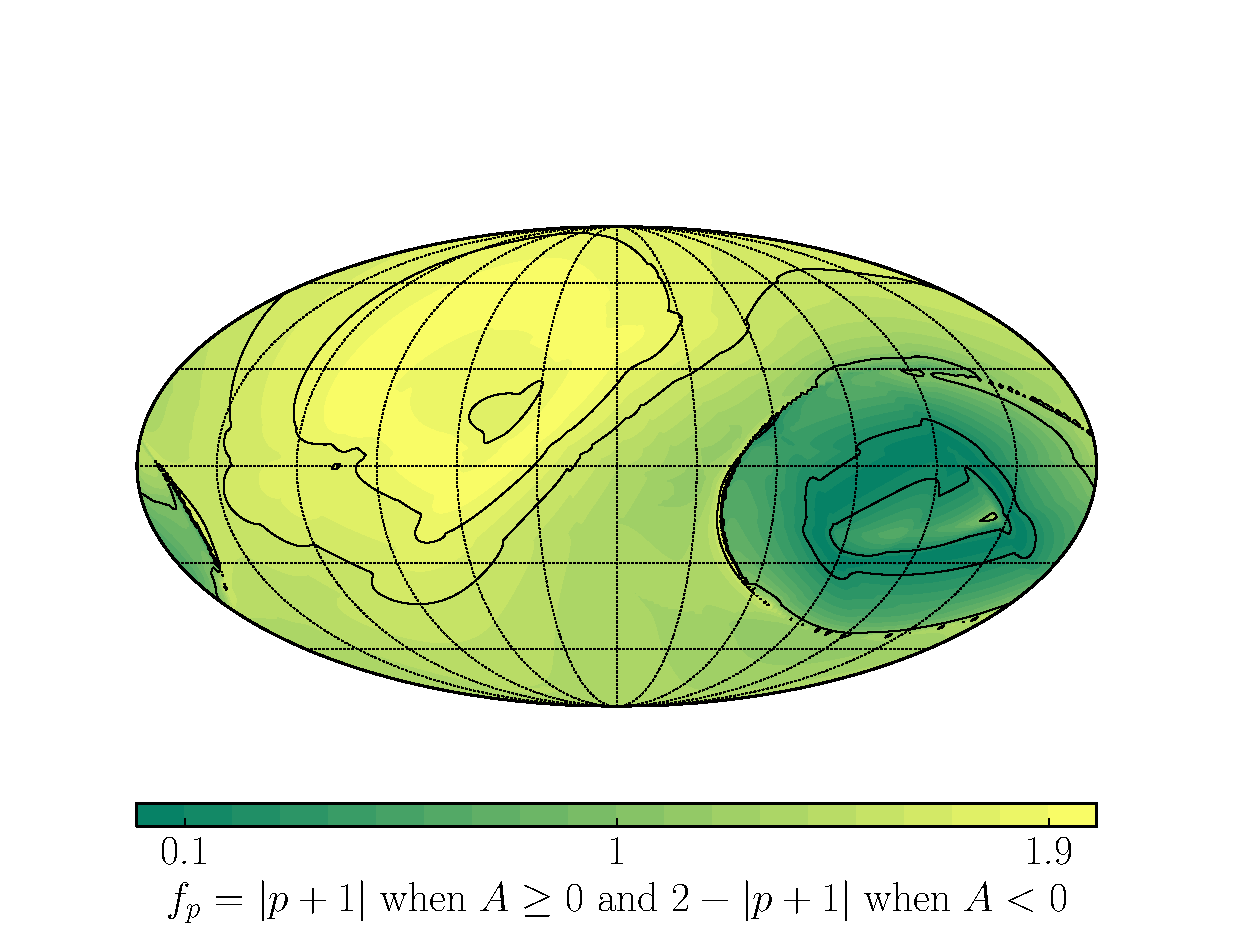
\includegraphics[width=0.8\textwidth]{Figure_7_bad.eps}\label{fig:skymap}
\caption{The value of $f_p$ across the sky that is sampled in Figure \ref{fig:hist_bad}, we can see why the sampled distribution does not have a well defined shape as the ``minimum" here is spread over a large region.  This is a boost of 400 km s$^{-1}$ using only primed shells (11 shells, 6.25 Mpc/$h$ inner cutoff) with respect to the LG.  The situation is much better when using unprimed shells, or both primed and unprimed.}
\end{figure}




\end{document}